\documentclass[tikz,border=5pt]{standalone}
\setlength{\voffset}{-1in}
\setlength{\hoffset}{-1in}
\usetikzlibrary{positioning}
\usetikzlibrary{shapes.geometric,calc}

% Parameters
\newcommand{\Frequency}{6.283185307}

% Variables
\newcommand{\PoleHeight}{1}
\newcommand{\PoleWidth}{.1}
\newcommand{\Ball}{0.9*\PoleWidth}
\newcommand{\s}{4.8}
\newcommand{\FlagPosTop}{.7*\PoleHeight}
\newcommand{\FlagThick}{30}
\newcommand{\FlagLength}{0.07}
\newcommand{\FlagAmplitude}{0.05}
\newcommand{\Periods}{\Frequency}
\newcommand{\Base}{3.0}
\newcommand{\CThick}{1.1}

% Fixed params
\newcommand{\CThickAdd}{0.1*\CThick - .1}
\newcommand{\BorderOffset}{0.007} % fixed
\newcommand{\ExtraPeriod}{0.065} % fixed
\newcommand{\FlagThickScaled}{0.0080337*\FlagThick} % fixed
\newcommand{\FlagPos}{.5*\PoleWidth} % fixed

\definecolor{Black}{RGB}{46, 46, 46}
\definecolor{LightBlue}{RGB}{118, 129, 216}
\definecolor{DarkBlue}{RGB}{86, 99, 208}
\definecolor{LightRed}{RGB}{170, 104, 96}
\definecolor{DarkRed}{RGB}{153, 70, 59}
\definecolor{LightGreen}{RGB}{140, 168, 98}
\definecolor{DarkGreen}{RGB}{114, 148, 63}
\definecolor{LightPurple}{RGB}{148, 123, 186}
\definecolor{DarkPurple}{RGB}{123, 91, 170}

\newcommand{\FlagColorLight}{LightRed}
\newcommand{\FlagColorDark}{DarkRed}

\newcommand{\BallColorLight}{LightBlue}
\newcommand{\BallColorDark}{DarkBlue}

\newcommand{\BaseColorLight}{LightPurple}
\newcommand{\BaseColorDark}{DarkPurple}

\begin{document}

\pagenumbering{gobble}
\noindent

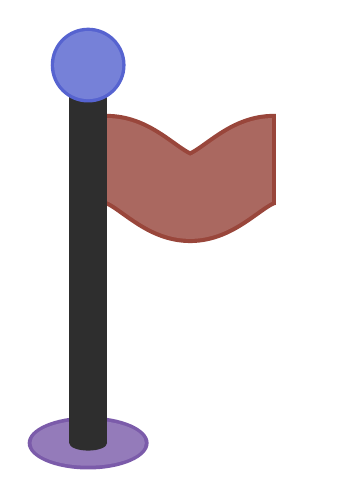
\begin{tikzpicture}[scale=\s]
  \tikzstyle{every node}=[font=\LARGE]
  % Flag
  \draw[domain = -\ExtraPeriod:\Periods+\ExtraPeriod,samples=100,line width=\CThick*\FlagThick, \FlagColorDark] plot(\x*\FlagLength+\FlagPos,{\FlagPosTop+\FlagAmplitude*cos(\x r)});
  \draw[domain = -\ExtraPeriod:\Periods+\ExtraPeriod,samples=100,line width=\FlagThick, \FlagColorLight]        plot(\x*\FlagLength+\FlagPos,{\FlagPosTop+\FlagAmplitude*cos(\x r)});
  \fill[\FlagColorDark] ({(\Periods+\ExtraPeriod)*\FlagLength+\FlagPos-\BorderOffset}, \FlagPosTop-.5*\FlagThickScaled+\FlagAmplitude) rectangle ++(\CThickAdd, \FlagThickScaled);

  % Base
  \fill[\BaseColorDark]   (0, 0) ellipse [x radius = {\CThickAdd+\Base*\FlagPos}, y radius = {\CThickAdd+\Base*.2*\PoleWidth}];
  \fill[\BaseColorLight]  (0, 0) ellipse [x radius = {\Base*\FlagPos}, y radius = {\Base*.2*\PoleWidth}];

  % Flag pole
  \fill[Black] ({-\FlagPos}, 0) rectangle ++(\PoleWidth,\PoleHeight);
  \fill[Black]      (0, 0) ellipse [x radius = {\FlagPos}, y radius = {.2*\PoleWidth}];

  % Flag ball
  \fill[\BallColorDark] (0,\PoleHeight) circle(\Ball*\CThick);
  \fill[\BallColorLight] (0,\PoleHeight) circle(\Ball);
\end{tikzpicture}

\end{document}